\let\negmedspace\undefined
\let\negthickspace\undefined
\documentclass[journal]{IEEEtran}
\usepackage[a4paper, margin=10mm, onecolumn]{geometry}
\usepackage{lmodern} % Ensure lmodern is loaded for pdflatex
\usepackage{tfrupee} % Include tfrupee package

\setlength{\headheight}{1cm} % Set the height of the header box
\setlength{\headsep}{0mm}  % Set the distance between the header box and the top of the text

\usepackage{gvv-book}
\usepackage{gvv}
\usepackage{cite}
\usepackage{amsmath,amssymb,amsfonts,amsthm}
\usepackage{algorithmic}
\usepackage{graphicx}
\usepackage{float}
\usepackage{textcomp}
\usepackage{xcolor}
\usepackage{txfonts}
\usepackage{listings}
\usepackage{enumitem}
\usepackage{mathtools}
\usepackage{gensymb}
\usepackage{comment}
\usepackage[breaklinks=true]{hyperref}
\usepackage{tkz-euclide} 
\usepackage{listings}
% \usepackage{gvv}                                        
\def\inputGnumericTable{}                                 
\usepackage[latin1]{inputenc}                                
\usepackage{color}                                            
\usepackage{array}                                            
\usepackage{longtable}                                       
\usepackage{calc}                                             
\usepackage{multirow}                                         
\usepackage{hhline}                                           
\usepackage{ifthen}                                           
\usepackage{lscape}
\usepackage{tikz}
\usetikzlibrary{patterns}

\begin{document}

\bibliographystyle{IEEEtran}
\vspace{3cm}

\title{5.5.16}
\author{EE25BTECH11064 - Yojit Manral}

\maketitle
% \maketitle
% \newpage
% \bigskip
{\let\newpage\relax\maketitle}
\renewcommand{\thefigure}{\theenumi}
\renewcommand{\thetable}{\theenumi}
\setlength{\intextsep}{10pt} % Space between text and float

\textbf{Question:}\\
\begin{align}
    \vec{A} = \myvec{2&-3&5\\3&-2&-4\\1&1&-2}
\end{align}
Find $\vec{A}^{-1}$. Use it to solve the given system of equations
\begin{align}
2x - 3y + 5z = 11 \\
3x - 2y - 4z = -5 \\
x + y - 2z = -3
\end{align}

\textbf{Solution:}\\
$\rightarrow$ Using the properties of inverses
\begin{align}
    \vec{A} \vec{A}^{-1} &= \vec{I}_{3\times3} \\
    \myvec{2&-3&5\\3&-2&-4\\1&1&-2}\vec{A}^{-1} &= \myvec{1&0&0\\0&1&0\\0&0&1}
\end{align}
$\rightarrow$ Now, using augmented matrix
\begin{align}
\left(\begin{array}{ccc|ccc} 2&-3&5&1&0&0\\3&-2&-4&0&1&0\\1&1&-2&0&0&1 \end{array}\right)
&\xrightarrow{R_1 \leftrightarrow (1/2)R_1} \left(\begin{array}{ccc|ccc} 1&-3/2&5/2&1/2&0&0\\3&-2&-4&0&1&0\\1&1&-2&0&0&1 \end{array}\right) \\
&\xrightarrow{R_2 \leftrightarrow R_2 - 3R_1} \left(\begin{array}{ccc|ccc} 1&-3/2&5/2&1/2&0&0\\0&5/2&-23/2&-3/2&1&0\\1&1&-2&0&0&1 \end{array}\right) \\
&\xrightarrow{R_3 \leftrightarrow R_3 - R_1} \left(\begin{array}{ccc|ccc} 1&-3/2&5/2&1/2&0&0\\0&5/2&-23/2&-3/2&1&0\\0&5/2&-9/2&-1/2&0&1 \end{array}\right) \\
&\xrightarrow{R_3 \leftrightarrow R_3 - R_2} \left(\begin{array}{ccc|ccc} 1&-3/2&5/2&1/2&0&0\\0&5/2&-23/2&-3/2&1&0\\0&0&7&1&-1&1 \end{array}\right) \\
&\xrightarrow{R_2 \leftrightarrow (2/5)R_2} \left(\begin{array}{ccc|ccc} 1&-3/2&5/2&1/2&0&0\\0&1&-23/5&-3/5&2/5&0\\0&0&7&1&-1&1 \end{array}\right) \\
&\xrightarrow{R_3 \leftrightarrow (1/7)R_3} \left(\begin{array}{ccc|ccc} 1&-3/2&5/2&1/2&0&0\\0&1&-23/5&-3/5&2/5&0\\0&0&1&1/7&-1/7&1/7 \end{array}\right) \\
&\xrightarrow{R_1 \leftrightarrow R_1 + (3/2)R_2} \left(\begin{array}{ccc|ccc} 1&0&-22/5&-2/5&3/5&0\\0&1&-23/5&-3/5&2/5&0\\0&0&1&1/7&-1/7&1/7 \end{array}\right) \\
&\xrightarrow{R_2 \leftrightarrow R_2 + (23/5)R_3} \left(\begin{array}{ccc|ccc} 1&0&-22/5&-2/5&3/5&0\\0&1&0&2/35&-9/35&23/35\\0&0&1&1/7&-1/7&1/7 \end{array}\right) \\
&\xrightarrow{R_1 \leftrightarrow R_1 + (22/5)R_3} \left(\begin{array}{ccc|ccc} 1&0&0&8/35&-1/35&22/35\\0&1&0&2/35&-9/35&23/35\\0&0&1&1/7&-1/7&1/7 \end{array}\right) \\
\implies \vec{A}^{-1} &= \frac{1}{35}\myvec{8&-1&22\\2&-9&23\\5&-5&5}
\end{align}
$\rightarrow$ From (2), (3) and (4), we get
\begin{align}
    \myvec{2&-3&5\\3&-2&-4\\1&1&-2} \myvec{x\\y\\z} &= \myvec{11\\-5\\-3} \\
    \vec{A}\hspace{1cm}\vec{x}\hspace{0.15cm} & \hspace{0.65cm}\vec{B} \notag
\end{align}
$\rightarrow$ So, we compute
\begin{align}
    \vec{x} &= \vec{A}^{-1} \vec{B} \\
    \vec{x} &= \frac{1}{35}\myvec{8&-1&22\\2&-9&23\\5&-5&5}\myvec{11\\-5\\-3} \\
    \vec{x} &= \myvec{27/35\\-2/35\\13/7}
\end{align}
\begin{figure}[h!]
   \centering
   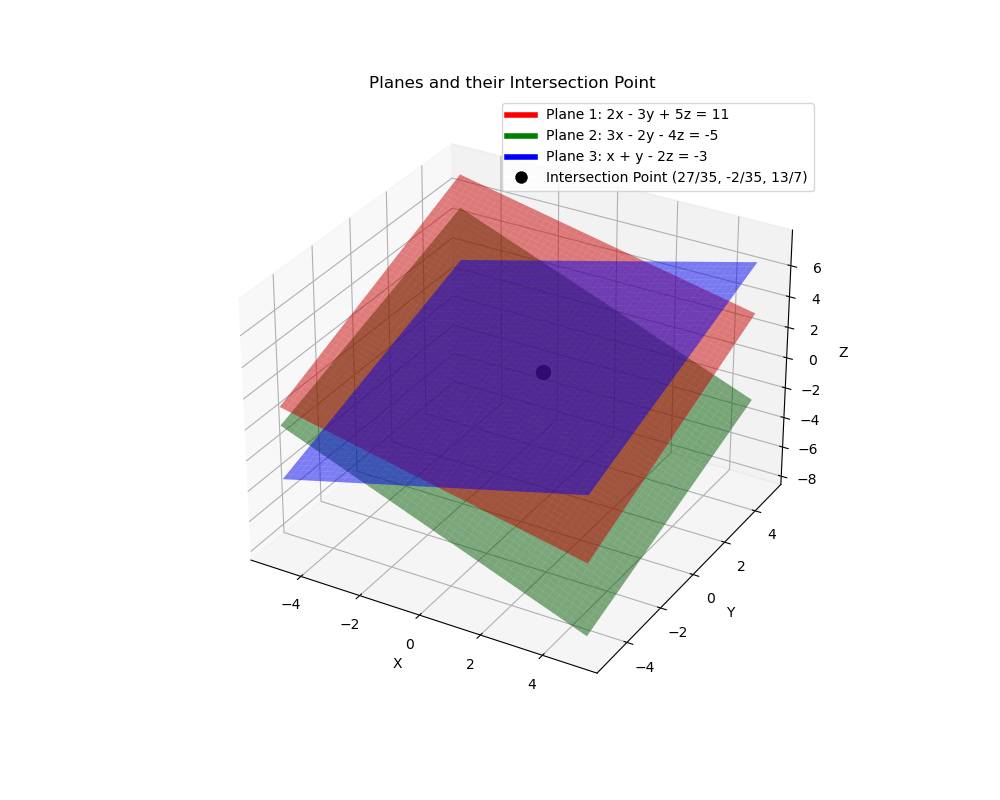
\includegraphics[width=\linewidth]{figs/01.png}
   \caption{Plot of system of equations}
   \label{Plot_1}
\end{figure}
\end{document}
